\chapter[ಅಧ್ಯಾಯ 8]{}\label{chap8}

\begin{center}
\rule{5cm}{1pt}\\[5pt]
{\Large\bfseries ಸಮಸ್ಯೆಗಳು}\\[3pt]
\rule{5cm}{1pt}
\end{center}

\begin{enumerate}
\renewcommand{\labelenumi}{\bf\theenumi.}
\itemsep=5pt

\item 1 2 3 4 5 6 7 8 9 = 100

$+$, $-$ ಇವುಗಳನ್ನು ಅಂಕಿಗಳ ನಡುವೆ ಹಾಕಿ ಸಮೀಕರಣ ಸರಿದೂಗಿಸಿ. ಅಂಕಿಗಳ ಕ್ರಮ ಬದಲಿಸಬಾರದು ಎರಡಂಕಿ, ಮೂರಂಕಿಗಳ ಗುಂಪು ಇರಬಹುದು. 

\item ಯಾವ ಎರಡು ಸಂಖ್ಯೆಗಳು ಗುಣಿಸಿದಾಗ ಬರುವ ಲಬ್ಧಕ್ಕಿಂತ ಭಾಗಿಸಿದಾಗ ಬರುವ ಲಬ್ಧ ಜಾಸ್ತಿ ಬರುತ್ತದೆ. 

\item 8 ಎಂಟು ಬಳಸಿ 8 ಬರಿಸಿ. ದಶಮಾಂಶ ನಿಷೇಧ :

\item ಒಂದೇ ಅಂಕಿಯನ್ನು ಮೂರು ಸಲ ಬಳಸಿ 24 ಬರಿಸಿ. 8ನ್ನು ಹೊರ ಪಡಿಸಿದೆ. ಯಾವುದೇ ಗಣಿತ ಪ್ರಕ್ರಿಯೆ ಬಳಸಬಹುದು. 

\item $4 + 4 + 4 + 4 = 452$. ಒಂದು ಚಿಕ್ಕ ಗೆರೆ ಸೇರಿಸಿ, ಸಮೀಕರಣ ಸರಿದೂಗಿಸಿ. $\neq$ ಬರುವಂತಿಲ್ಲ. 

\item $2 + 2 = 4 ~~;~~ 2\times 2 = 4$. ಇಂತಹ ಬೇರೆ ಉದಾಹರಣೆ ಕೊಡಿ. ಭಿನ್ನರಾಶಿ ಬಳಸಬಹುದು. 

\item ಒಂದು ಸಂಖ್ಯೆಯ $\frac{2}{3}$ರಷ್ಟನ್ನು 24ಕ್ಕೆ ಸೇರಿಸಿದರೆ 36 ಬರುತ್ತದೆ. ಸಂಖ್ಯೆ ಯಾವುದು? 

\item ಇದೊಂದು ವಿಚಿತ್ರ. ಯಾವುದಾದರೂ ಸಂಖ್ಯೆಯನ್ನು ಇಂಗ್ಲಿಷ್ ಭಾಷೆಯಲ್ಲಿ\break ಬರೆಯಿರಿ. ಅಕ್ಷರಗಳನ್ನು ಎಣಿಸಿ. ಮೊತ್ತವನ್ನು ಇಂಗ್ಲಿಷ್‌ನಲ್ಲಿ ಬರೆಯಿರಿ. ಪ್ರಕ್ರಿಯೆ ಮುಂದುವರಿಸಿ. ಅಂತಿಮ ಉತ್ತರ ಯಾವಾಗಲೂ FOUR.

\item ಎಂಟು 8 ಬಳಸಿ 1000 ಬರಿಸಿ. ಯಾವುದೇ ಗಣಿತ ಪ್ರಕ್ರಿಯೆ ಬಳಸಬಹುದು. 

\item ಮೂರು 9 ಬಳಸಿ 1  ಬರಿಸಿ. ಯಾವುದೇ ಗಣಿತ ಪ್ರಕ್ರಿಯೆ ಬಳಸಬಹುದು. 

\item ಒಂದು/ಹೆಚ್ಚು ಗೆರೆ ಸ್ಥಾನ ಪಲ್ಲಟ ಮಾಡಿ ಸಮೀಕರಣ ಸರಿದೂಗಿಸಿ $\neq$ ಬರುವಂತಿಲ್ಲ. 
\begin{itemize}
\item[(a)] VI = II
\item[(b)] I $-$ III = II
\item[(c)] X $-$ I = I
\item[(d)] XI $+$ 0 = I
\end{itemize}

\item 6 ಮತ್ತು 6 ಸೇರಿಸಿ 11 ಬರಿಸಿ. 

\item 24 ಬೆಂಕಿಕಡ್ಡಿ ಜೋಡಿಸಿ $3\times 3$ ಚೌಕಾಕೃತಿ ರಚಿಸಿದೆ. 
\begin{figure}[H]
\centering
\includegraphics{images/chap8/q13.eps}
\end{figure}

\begin{itemize}
\item[(a)] 12 ಕಡ್ಡಿ ಸ್ಥಾನ ಪಲ್ಲಟ ಮಾಡಿ 2 ಸಮಾನ ಅಳತೆಯ ಚೌಕ ಬರಿಸಿ.
\item[(b)] 4 ಕಡ್ಡಿ ತೆಗೆದು ಹಾಕಿ, 4 ಚಿಕ್ಕ ಮತ್ತು 1 ದೊಡ್ಡ ಚೌಕ ಬರಿಸಿ.
\item[(c)] 6 ಕಡ್ಡಿ ತೆಗೆದು ಹಾಕಿ 3 ಚೌಕ ಬರಿಸಿ.
\item[(d)] 8 ಕಡ್ಡಿ ತೆಗೆದು ಹಾಕಿ 4 ಚೌಕ ಬರಿಸಿ.
\item[(e)] 8 ಕಡ್ಡಿ ತೆಗೆದು ಹಾಕಿ 2 ಚೌಕ ಬರಿಸಿ.
\item[(f)] 8 ಕಡ್ಡಿ ತೆಗೆದು ಹಾಕಿ 3 ಚೌಕ ಬರಿಸಿ.
\item[(g)] 6 ಕಡ್ಡಿ ತೆಗೆದು ಹಾಕಿ 2 ಚೌಕ, 2 `L' ಆಕಾರದ ಆಕೃತಿ ಬರಿಸಿ 
\item[(h)] 4, 6, 8 ಕಡ್ಡಿಗಳನ್ನು ತೆಗೆದು ಹಾಕಿದಾಗ ಪ್ರತಿ ಬಾರಿಯೂ 5 ಚೌಕ (1 ಕಡ್ಡಿ ಬಾಹು) ಇರುವಂತೆ ರಚಿಸಿ. 
\end{itemize}

\item ಈ ಗುಣಾಕಾರ ಗಮನಿಸಿ ಮುಂದಿನ 3 ಹಂತ ಬರೆಯಿರಿ.

\begin{tabular}[t]{c@{\;}c@{\;}c}
$7\times 7$ & = & $49$\\
$67\times 67$ & = & $4489$\\
$667\times 667$ & = & $444889$
\end{tabular}


\item ಈ ಗುಣಾಕಾರ ಗಮನಿಸಿ ಮುಂದಿನ 6 ಹಂತ ಬರೆಯಿರಿ. 

\begin{tabular}[t]{c@{\;}c@{\;}c}
222 ~ 222 ~ 222 $\times$ 9 & = & 1 ~~ 999 ~ 999 ~ 998\\
333 ~ 333 ~ 333 $\times$ 9 & = & 2 ~~ 999 ~ 999 ~ 997\\
444 ~ 444 ~ 444 $\times$ 9 & = & 3 ~~ 999 ~ 999 ~ 996
\end{tabular}

\item ಈ ಗುಣಾಕಾರದಲ್ಲಿ 1 ರಿಂದ 9ವರೆಗಿನ ಅಂಕಿಗಳು ಒಮ್ಮೆ ಮಾತ್ರ ಬಂದಿದೆ. ಇಂತಹ ಇನ್ನೆರಡು ಉದಾಹರಣೆ ಕೊಡಿ. $\qquad 48\times 159 = 7632$


\item ಒಂದು ಸಂಖ್ಯೆಯನ್ನು ಎಡದಿಂದ ಬಲಕ್ಕೆ ಅಥವಾ ಬಲದಿಂದ ಎಡಕ್ಕೆ ಓದಿದಾಗ\break ಒಂದೇ ರೀತಿ ಇದ್ದರೆ ಅದು ``ಮಾಲಾ ಸಂಖ್ಯೆ" (Palindrome number)

ಇವುಗಳನ್ನು ಗುಣಾಕಾರದಲ್ಲಿ ಪಡೆಯಲು ಹಲವು ವಿಧಾನಗಳಿವೆ. 

\begin{tabular}[t]{c@{\;}c@{\;}l}
$12\times 21$ & = & $252$\\
$112\times 211$ & = & $23632$\\
$1112\times 2111$ & = & $2347432$
\end{tabular}

\vskip 0.1cm

ಮುಂದಿನ 3 ಹಂತ ಬರೆಯಿರಿ. 

\item ಬೇರೆ ಬೇರೆ ಅಳತೆಯ 8 ರೇಖಾ ಖಂಡ ಬಳಸಿ, ಬೇರೆ ಬೇರೆ ಅಳತೆಯ, ಪರಸ್ಪರ ಲಗತ್ತಾಗಿರುವ 3 ಚೌಕ ಬರಿಸಿ.

\item ಎಷ್ಟು $\frac{1}{4}$ `` ಚೌಕಗಳು 1" ಚೌಕ ಮಾಡುತ್ತವೆ? 

\item ಈ ಆಕೃತಿ ಗಮನಿಸಿ. ಅದರಲ್ಲಿರುವ ಎಲ್ಲಾ ಅಳತೆಯ ತ್ರಿಭುಜಗಳು ಒಟ್ಟು ಎಷ್ಟು? 

\begin{figure}[H]
\centering
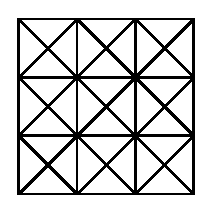
\includegraphics[scale=1.3]{images/chap8/q20.eps}
\end{figure}

\vskip -0.4cm

\item ಆದ್ಯೇ ದಿನೇ ದ್ರಮ್ಮ ಚತುಷ್ಟಯಂ ಯೋದತ್ವಾದ್ವಿಜೇಭ್ಯೋನುದಿನಂ ಪ್ರವೃತ್ತಃ 

ದಾತುಂ ಸಖೇ ಪಂಚ ಚಯೇನಪಕ್ಷೇದ್ರಮ್ಮಾವದ ದ್ರಾಕ್ವನಿತೇನದತ್ತಾಃ ।


{\bf ಅರ್ಥ:} ಒಬ್ಬ ರಾಜನು 15 ದಿನಗಳ ಕಾಲ ಬ್ರಾಹ್ಮಣರಿಗೆ ಹಣದಾನ ಮಾಡಿದನು ಮೊದಲ ದಿನ 4 ದ್ರಮ್ಮ (ಒಂದು ನಾಣ್ಯ)ಗಳನ್ನು ಕೊಟ್ಟನು. ಎರಡನೆದಿನ 9, ಮೂರನೆದಿನ 14 ಹೀಗೆ ಐದೈದು ಹೆಚ್ಚಿಸಿದನು. ಅವನು ದಾನ ಮಾಡಿದ ದ್ರಮ್ಮಗಳೆಷ್ಟು? 

\item 1, 3, 5, 7, 9, 11, 13, 15 ಇವು ಕ್ರಮಾಗತ ಬೆಸ ಸಂಖ್ಯೆಗಳು. ಇವುಗಳಲ್ಲಿ ಯಾವುದಾದರೂ 5 ಸಂಖ್ಯೆಗಳನ್ನು ಈ ಕೆಳಗಿನ ಕೋಷ್ಠಗಳಲ್ಲಿ ತುಂಬಿಸಿ, ಸಮೀಕರಣ ಸರಿದೂಗಿಸಿ. 

$\Box + \Box + \Box + \Box + \Box = 30$

ಸಂಖ್ಯೆಗಳನ್ನು ಪುನರಾವರ್ತಿಸಬಹುದು. 

\{ಇದು ಸ್ಪರ್ಧಾತ್ಮಕ ಪರೀಕ್ಷೆಯಲ್ಲಿ ಕೇಳಿದ ಪ್ರಶ್ನೆ. ಗಣಿತೀಯ ಉತ್ತರ ಸಾಧ್ಯವಿಲ್ಲ. ತಾರ್ಕಿಕ ಉತ್ತರದ ಬಗ್ಗೆ ಆಲೋಚಿಸಿ\}

\item ಯಾವುದೇ 3ರ ಗುಣಕ ತೆಗೆದುಕೊಳ್ಳಿ. 

ಉದಾ: 9 ಅದರ ಘನ ಬರೆಯಿರಿ. $9^{3} = 729$

ಅಂಕಿಗಳ ಘನ ಬರೆದು ಮೊತ್ತ ಬರೆಯಿರಿ. 

$7^{3} + 2^{2} + 9^{3} = 343 + 8 + 729 = 1080$

ಪ್ರಕ್ರಿಯೆ ಮುಂದುವರಿಸಿ $1^{2} + 0^{3} + 8^{3} + 0^{2} = 1 + 512 = 513$

ಘನ $5^{3} + 1^{3} + 3^{3} = 125 + 1 + 27 = 153$

ಯಾವುದೇ 3ರ ಗುಣಕದಿಂದ ಪ್ರಾರಂಭಿಸಿದರೂ ಅಂತಿಮ ಉತ್ತರ 153

ಬೇರೆ ಸಂಖ್ಯೆಗಳಿಂದ ಯತ್ನಿಸಿ. 

\item ಪೆನ್ಸಿಲ್ಲನ್ನು ಮೇಲೆತ್ತದೆ, ಒಂದೇ ರೇಖೆಯ ಮೇಲೆ 2 ಬಾರಿ ಹೋಗದೆ, ಹಿಮ್ಮುಖ ಚಲನೆಯಿಲ್ಲದೆ, ಈ ಆಕೃತಿಯ ಎಲ್ಲ ರೇಖೆಗಳ ಮೇಲೂ ಚಲಿಸಿ. 
\begin{figure}[H]
\centering
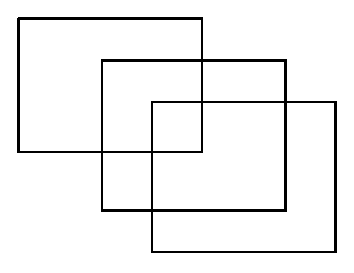
\includegraphics{images/chap8/q24.eps}
\end{figure}

\item ಒಬ್ಬ ಧನಿಕ ಮಹಾಜಿಪುಣ, ಹಣ ಸಂಪಾದಿಸುವದೊಂದೇ ಗುರಿ. ಗಣಿತದಲ್ಲಿ ಬಾರೀ ದಡ್ಡ. ಒಬ್ಬ ಗಣಿತಜ್ಞ ಕಿಲಾಡಿ, ಬಡವ. ಧನಿಕನ ಪರಿಚಿತ. ಒಂದು ದಿನ ಕಿಲಾಡಿ ಧನಿಕನಿಗೆ ಹೇಳಿದ. ``ನೀವು ಒಪ್ಪುವುದಾದರೆ ಒಂದು ಆಟ ಆಡೋಣ". ಧನಿಕ ಏನು ಆಟ ಎಂದ. ಕಿಲಾಡಿ ಹೇಳಿದ: ``ನಾನು 1 ತಿಂಗಳ ಕಾಲ ದಿನವೂ ನಿಮಗೆ 1 ಲಕ್ಷರೂ ಕೊಡುತ್ತೇನೆ. ನೀವು ನನಗೆ ಮೊದಲದಿನ 1ರೂ, 2ನೆ ದಿನ 2ರೂ, ಮೂರನೆ ದಿನ 4ರೂ ಹೀಗೆ ಎರಡರಷ್ಟು ಮಾಡಿ ತಿಂಗಳು ಪೂರ್ತ ಕೊಡಬೇಕು". ಧನಿಕ ಸಂತೋಷದಿಂದ ಒಪ್ಪಿದ ಈ ವ್ಯವಹಾರದಲ್ಲಿ ಯಾರಿಗೆ ಲಾಭ, ಯಾರಿಗೆ ನಷ್ಟ? 

\item ಯಾವ ಸಂಖ್ಯೆಯ ವರ್ಗವನ್ನು 32ರಿಂದ ಗುಣಿಸಿ 1ನ್ನು ಕೂಡಿಸಿದರೆ ಇನ್ನೊಂದು ವರ್ಗಸಂಖ್ಯೆ ಲಭಿಸುತ್ತದೆ? 

\item ಒಂದು ಕುಟುಂಬದಲ್ಲಿ ಗಂಡು ಮಕ್ಕಳು, ಹೆಣ್ಣು ಮಕ್ಕಳು ಇದ್ದಾರೆ. ಒಬ್ಬ ಹುಡುಗನನ್ನು ನೀವೆಷ್ಟು ಸಹೋದರ$-$ಸಹೋದರಿಯರು ಎಂದು ಕೇಳಿದರೆ ``ನನಗೆ ಇರುವ ಸಹೋದರ$-$ಸಹೋದರಿಯರ ಸಂಖ್ಯೆ ಸಮ" ಎಂದು ಉತ್ತರ. ಒಬ್ಬಳು ಹುಡುಗಿಯನ್ನು ಅದೇ ಪ್ರಶ್ನೆ ಕೇಳಿದಾಗ ``ಸಹೋದರಿಯರ ಸಂಖ್ಯೆಯ 2ರಷ್ಟು ಸಹೋದರರು" ಉತ್ತರ. ಕುಟುಂಬದ ಗಂಡು ಮಕ್ಕಳ, ಹೆಣ್ಣು ಮಕ್ಕಳ ಸಂಖ್ಯೆ ಎಷ್ಟು? 

\item ಒಂದು ರೈಲು ಬಂಡಿ ಕಂಬವೊಂದನ್ನು ಹಾದು ಹಾದುಹೋಗಲು 9 ಸೆ. ತೆಗೆದುಕೊಳ್ಳುತ್ತದೆ. 88 ಮೀ ಉದ್ದದ ಪ್ಲಾಟ್ ಫಾರಂ ಹಾದು ಹೋಗಲು 21 ಸೆ. ಬೇಕು. ರೈಲಿನ ಉದ್ದವೆಷ್ಟು? 

\item 1, 6, 7, 9 ಇವುಗಳನ್ನು ಒಮ್ಮೆ ಮಾತ್ರ ಬಳಸಿ 24 ಬರಿಸಿ. ಯಾವುದೇ ಗಣಿತೀಯ ಚಿಹ್ನೆ ಪ್ರಕ್ರಿಯೆ ಬಳಸಬಹುದು. ಎಲ್ಲ ಅಂಕಿಗಳನ್ನೂ ಬಳಸಲೇಬೇಕು. 

\item 1, 2, 3, 4, 5, 6 ಇವುಗಳಿಂದ ಭಾಗಿಸಲ್ಪಟ್ಟಾಗ 1 ಶೇಷ ಉಳಿಯುವ ಕನಿಷ್ಠ ಸಂಖ್ಯೆ ಯಾವುದು? 
\end{enumerate}

\smallskip

\begin{center}
\rule{5cm}{1pt}\\[3pt]
{\Large\bfseries ಉತ್ತರಗಳು}\\[-0.1cm]
\rule{5cm}{1pt}
\end{center}

\begin{enumerate}
\itemsep=5pt

\item ಎರಡು ಉತ್ತರಗಳಿವೆ. 
\begin{itemize}
\item[(a)] $1 + 2 + 3 - 4 + 5 + 6 +78 + 9 = 100$
\item[(b)] $123 - 45 - 67 + 89 = 100$
\end{itemize}

\item $\dfrac{1}{3} \div \dfrac{1}{3} = 1\quad;\quad \dfrac{1}{3} \times \dfrac{1}{3} = \dfrac{1}{9}$ ಯಾವುದೇ ಭಿನ್ನರಾಶಿಯಾಗಬಹುದು. 

\item $8(88888)^{8-8} = 8(88888)^{0} = 8\times 1 = 8$

\item 
\begin{align*}
8 + 8 + 8 & = 24\\
3^{3} - 3 & = 24\\
4!\quad +4 - 4 & = 24 \qquad\{4! = 4 \times 3 \times 2 \times 1\}
\end{align*}

\item  $4 + 444 + 4 = 452$

($+$ ಚಿಹ್ನೆಗೆ 1 ಚಿಕ್ಕಗೆರೆ ಸೇರಿಸಿ 4 ಮಾಡಿದೆ.)

\item ಯಾವುದೇ ಅಂಕಿ ಅಥವಾ ಸಂಖ್ಯೆ ಮತ್ತು ಅದರ ಹಿಂದಿನ ಅಂಕಿ ಅಥವಾ ಸಂಖ್ಯೆಯನ್ನು ಛೇದವಾಗಿಸಿ, ದತ್ತ ಸಂಖ್ಯೆಯನ್ನು ಅಂಶವಾಗುಳ್ಳ ಸಂಖ್ಯೆ $-$ ಇವು ಗುಣಿಸಿದಾಗ, ಕೂಡಿಸಿದಾಗ ಸಮಾನ ಉತ್ತರ ಲಭಿಸುತ್ತದೆ. 

ಉದಾ: $3, \dfrac{3}{2} \quad;\quad 3 \times \dfrac{3}{2} = 3 + \dfrac{3}{2} = \dfrac{9}{2} = 4\dfrac{1}{2}$
\begin{align*}
4, \dfrac{4}{3} \quad;\quad 4\times \dfrac{4}{3} & = 4 + \dfrac{4}{3} = 5\dfrac{1}{3}\\
10, \dfrac{10}{9} \quad;\quad 10\times \dfrac{10}{9} & = 10 + \dfrac{10}{9} = 11\dfrac{1}{9}
\end{align*}

\item ಸಂಖ್ಯೆ $x$ ಇರಲಿ 

\vskip 0.1cm
$\dfrac{2}{3}$ರಷ್ಟು $\dfrac{2x}{3}$

\vskip 0.1cm
24ಕ್ಕೆ ಸೇರಿಸಿ $24 + \dfrac{2x}{3}$

\vskip 0.1cm
ಸಮೀಕರಣ $24 + \dfrac{2x}{3} = 36$

\vskip 0.1cm
$\dfrac{2x}{3} = 36 - 24 \quad;\quad \dfrac{2x}{3} =12 ~~;~~ 2x = 36$

\vskip 0.1cm
$x = 18$

\item ಉದಾ: 

\begin{tabular}[t]{llll}
FOURTEEN & 8 ಅಕ್ಷರಗಳು & ONE & 3 ಅಕ್ಷರಗಳು\\
EIGHT & 5 ಅಕ್ಷರಗಳು  & THREE & 5 ಅಕ್ಷರಗಳು\\
FIVE & 4 ಅಕ್ಷರಗಳು  & FIVE & 4 ಅಕ್ಷರಗಳು\\
FOUR & 4 ಅಕ್ಷರಗಳು  & FOUR & 4 ಅಕ್ಷರಗಳು
\end{tabular}

\vskip 0.2cm

\begin{tabular}[t]{ll}
TWO HUNDRED SEVENTY ONE & 20 ಅಕ್ಷರಗಳು\\
TWENTY & 6 ಅಕ್ಷರಗಳು\\
SIX & 3 ಅಕ್ಷರಗಳು\\
THREE & 5 ಅಕ್ಷರಗಳು\\
FIVE & 4 ಅಕ್ಷರಗಳು\\
FOUR & 4 ಅಕ್ಷರಗಳು
\end{tabular}

\smallskip
\item 
\begin{itemize}
\item[(a)] $\dfrac{8888 - 888}{8} = 1000$
\item[(b)] $\left(8 + \dfrac{8 + 8}{8}\right)^{\dfrac{8+8+8}{8}} = \left(8 + \dfrac{16}{8}\right)^{\dfrac{24}{8}}$

\smallskip

$= (8 + 2)^{3} = 10^{3} = 1000$
\item[(c)] 
\begin{align*}
& 8(8\times 8 + 8\times 8) - 8 - 8 - 8\\
& = 8(64 + 64) - 24\\
& = 8(128) - 24 = 1024 - 24 = 1000
\end{align*}
\end{itemize}

\item $9^{9-9} = 9^{0} = 1$

\item 
\begin{itemize}
\item[(a)] $\sqrt{1} = 1$ \{11 ರ ಒಂದು ಗೆರೆಯನ್ನು ಅಡ್ಡಲಾಗಿಸಿದೆ\}
\item[(b)] I = III $-$ II \{II ನ ಒಂದು ಗೆರೆಯನ್ನು ಮೊದಲ 1ರ ಹಿಂದೆ ಬರೆದಿದೆ\}
\item[(c)] $1\times 1 = 1$ \{$-$ ಗೆರೆಯನ್ನು ನೇರ ಮಾಡಿ $\times$ ನ ಹಿಂದೆ ಬರೆದಿದೆ\}
\item[(d)] XI $-$ 10 = 1 \{$+$ನ 1 ಗೆರೆಯನ್ನು 0ಯ ಹಿಂದೆ ಬರೆದಿದೆ.\}
\end{itemize}

\eject

\item VI, VI ಎರಡು 6ಗಳು 

\begin{tabular}[t]{ll}
VI & \multirow{2}{*}{= {\rm XI} \{ಒಂದು 6ನ್ನು ತಲೆಕೆಳಗು ಮಾಡಿ ಇನ್ನೊಂದರ ಕೆಳಗೆ ಬರೆದಿದೆ\}}\\[-7pt]	
${\rotatebox{180}{IV}}$ &\\
\end{tabular}

\item ಇದು ಕೊಟ್ಟಿರುವ ಜೋಡಣೆ ಇರಲಿ 
\begin{figure}[H]
\centering
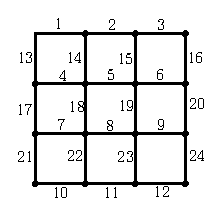
\includegraphics[scale=1.2]{images/chap8/ans13.eps}
\end{figure}


\begin{figure}[H]
\centering
\includegraphics[scale=1.1]{images/chap8/ans13a.eps}
\end{figure}

\begin{minipage}[c]{4.5cm}
\begin{figure}[H]
\centering
\includegraphics{images/chap8/ans13b.eps}

\text{5, 8, 19, 18 ಕಡ್ಡಿ ತೆಗೆದಿದೆ.}
\end{figure}
\end{minipage}
\begin{minipage}[c]{4.5cm}
\begin{figure}[H]
\centering
\includegraphics{images/chap8/ans13c.eps}

\text{14, 15, 4, 7, 8, 19 ತೆಗೆದಿದೆ}
\end{figure}
\end{minipage}


\begin{figure}[H]
\centering
\text{ಎರಡು ಉತ್ತರಗಳಿವೆ }

\includegraphics{images/chap8/ans13d.eps}

\text{2, 5, 17, 18, 19, 20, 8, 11 ಕಡ್ಡಿ ತೆಗೆದಿದೆ \quad 2, 3, 15, 16, 17, 20, 6, 11 ಕಡ್ಡಿ ತೆಗೆದಿದೆ }
\end{figure}

\begin{minipage}[c]{4cm}
\begin{figure}[H]
\centering
\includegraphics{images/chap8/ans13e.eps}
\end{figure}
\end{minipage}
\qquad
\begin{minipage}[c]{4cm}
\begin{equation*}
\left.
\begin{aligned}
14, 15\\
4, 6\\
7, 9\\
22, 23
\end{aligned}
\right\}
\text{ಒಟ್ಟು  8 ಕಡ್ಡಿ ತೆಗೆದಿದೆ}
\end{equation*}
\end{minipage}

\begin{minipage}[c]{4cm}
\begin{figure}[H]
\centering
\includegraphics{images/chap8/ans13f.eps}
\end{figure}
\end{minipage}
\begin{minipage}[c]{5cm}
\begin{equation*}
\left.
\begin{aligned}
5, 15, 6, 19\\
8, 22, 7, 18
\end{aligned}
\right\}
\text{ತೆಗೆದಿದೆ}
\end{equation*}
\end{minipage}

\begin{minipage}[c]{4cm}
\begin{figure}[H]
\centering
\includegraphics{images/chap8/ans13g.eps}
\end{figure}
\end{minipage}
\begin{minipage}[c]{5cm}
\begin{equation*}
\left.
\begin{aligned}
14, 15\\
6, 7\\
22, 23
\end{aligned}
\right\}
\text{ತೆಗೆದಿದೆ}
\end{equation*}
\end{minipage}
\begin{figure}[H]
\centering
\includegraphics{images/chap8/ans13h.eps}
\end{figure}


\item 
\begin{tabular}[t]{ccc}
$6667\times 6667$ & = & $44448889$\\[0.1cm]
$66667\times 66667$ & = & $4444488889$\\[0.1cm]
$666667\times 666667$ & = & $444444888889$
\end{tabular}


\item 
\begin{tabular}[t]{llllllll}
$555$ & $555$ & $555\times 9$ & = & $4$ & $999$ & $999$ & $995$\\
$666$ & $666$ & $666\times 9$ & = & $5$ & $999$ & $999$ & $994$\\
$777$ & $777$ & $777\times 9$ & = & $6$ & $999$ & $999$ & $993$\\
$888$ & $888$ & $888\times 9$ & = & $7$ & $999$ & $999$ & $992$\\
$999$ & $999$ & $999\times 9$ & = & $8$ & $999$ & $999$ & $991$
\end{tabular}

\item 
\begin{tabbing}
$42\times 138$ \= =  $5796$\\
$157\times 28$ \> = $4396$
\end{tabbing}

\item 
\begin{tabular}[t]{ccc}
$11112\times 21111$ & = & $234585432$\\
$111112\times 211111$ & = & $23456965432$\\
$1111112\times 2111111$ & = & $2345679765432$
\end{tabular}



\item 3 ಚೌಕಗಳು 8 ರೇಖಾಕಂಡಗಳು 
\begin{figure}[H]
\centering
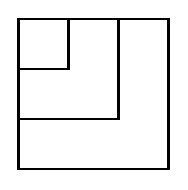
\includegraphics[scale=0.9]{images/chap8/ans18.eps}
\end{figure}


\item 16 ಚೌಕಗಳು 

\item 150 ತ್ರಿಭುಜಗಳು 

\item ದಾನ ಮಾಡಿದ ಹಣ $4 + 9 + 14 + \cdots 15$ ಸಂಖ್ಯೆಗಳು. ಇದು ಅಂಕಗಣಿತ ಶ್ರೇಣಿಯ ಲೆಕ್ಕ 

ಮೊದಲ ಪದ 4, ಚಯ (common difference)5, ಪದಗಳು 15

ಅಂತ್ಯ ಪದ $(15 - 1)\times 5 + 4 = 74$

\vskip 0.1cm

ಮಧ್ಯ ಪದ $\dfrac{74 + 4}{2} = 39$

\vskip 0.1cm

ಒಟ್ಟು ಧನ $= 39\times 15 = 585$ ದ್ರಮ್ಮುಗಳು 

\item ಎರಡು ಬೆಸ ಸಂಖ್ಯೆಗಳ ಮೊತ್ತ ಯಾವಾಗಲೂ ಸಮ ಸಂಖ್ಯೆ 4 ಬೆಸ ಸಂಖ್ಯೆಗಳ ಮೊತ್ತವೂ ಸಮ ಸಂಖ್ಯೆ. $\therefore$ 5 ಬೆಸ ಸಂಖ್ಯೆಗಳ ಮೊತ್ತ ಬೆಸ ಸಂಖ್ಯೆ. ಕೊಟ್ಟಿರುವ ಮೊತ್ತ 30 ಸಮ ಸಂಖ್ಯೆ 

$\therefore$ ಗಣತೀಯ ಉತ್ತರ ಅಸಾಧ್ಯ 

\vskip 0.2cm

\begin{tabular}{c@{\;}c@{\;}c@{\;}c@{\;}c@{\;}c@{\;}c@{\;}c@{\;}c@{\;}c@{\;}c}
\fbox{3} &+& \fbox{7}& + &\fbox{11}& +& \fbox{13}& +& \fbox{1} & = & 30\\
ವಾರ & & ದಿನ & & ಗಂಟೆ & & ಗಂಟೆ & & ದಿನ & & \\[-0.3cm]
&&&& \multicolumn{3}{m{2cm}}{$\underbrace{\hspace{1.5cm}}$}&&&\\
21 & & 7 & & & 1 & & & 1 & = & 30 ದಿನ 
\end{tabular}

\item ಉತ್ತರದ ಅಗತ್ಯವಿಲ್ಲ 

\item 
~

\begin{figure}[H]
\centering
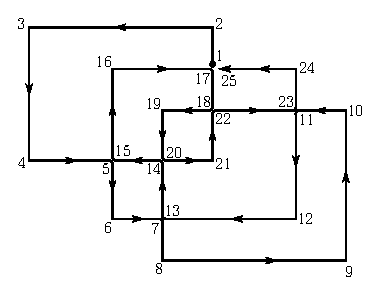
\includegraphics[scale=1.1]{images/chap8/ans24.eps}
\end{figure}

\eject

\item ಧನಿಕನಿಗೆ ಕಿಲಾಡಿ ಕೊಡುವ ಹಣ 1 ಲಕ್ಷ $\times$ 30 ದಿನ  = 30 ಲಕ್ಷ ರೂ.

ಧನಿಕ ಕಿಲಾಡಿಗೆ ಕೊಡುವ ಹಣ 
\begin{align*}
& 1+2+4+8+16+32+64+128+256+512+1024\\
& +2048+4096+8192+11384+32768+65536+\\
& 1,31,072+262144+5,24,288+1048576+20,97,152\\
& {18 \text{ ನೆ ದಿನ}} ~~~\quad {19 \text{ ನೆ ದಿನ}}\qquad {20 \text{ ನೆ ದಿನ}}\quad{21 \text{ ನೆ ದಿನ}}~~~\quad{22 \text{ ನೆ ದಿನ}}
\end{align*}

ಮುಂದಕ್ಕೆ ಲಕ್ಷದಿಂದ ಕೋಟಿಗೂ ಹೆಚ್ಚುತ್ತದೆ. ಕಿಲಾಡಿಗೆ ಹೆಚ್ಚು ಹಣ ಬರುತ್ತದೆ. 

\item  ಸಮೀಕರಣ ಹೀಗಿರುತ್ತದೆ. $32x^{2} + 1 = y^{2}$

$x=3$ ಆದಾಗ $y=17$ ಆಗುತ್ತದೆ. 

$32\times 9 = 288 + 1 = 289 = 17^{2}$

\item ಕುಟುಂಬದಲ್ಲಿ $x$ ಹುಡುಗರು $y$ ಹುಡುಗಿಯರು ಇರಲಿ 

ಒಬ್ಬ ಹುಡುಗ  $x - 1 = y$

ಒಬ್ಬ ಹುಡುಗಿ $(y - 1); 2(y - 1) = x$
\begin{tabbing}
$x - y$  =  $1$\\
$x - 2y$ =  $-1$
\end{tabbing}

\vskip -2cm

\begin{gather*}
\therefore\quad x  = y + 1\\
2(y - 1)  = y + 1\\
2y - 2  = y + 1\\
y  = 3\\
\therefore\quad x  = 4
\end{gather*}
4 ಹುಡುಗರು\quad 3 ಹುಡುಗಿಯರು 

\item ರೈಲಿನ ಉದ್ದ $x$ಮೀ. ಇರಲಿ 

\vskip 0.1cm

$x$ಮೀ. ಚಲಿಸಲು 9ಸೆ. 

\vskip 0.1cm

$\therefore\quad 1$ ಸೆಕೆಂಡಿಗೆ $\dfrac{x}{9}$ ಮೀ. 

\vskip 0.1cm

$(x+88)$ಮೀ ಉದ್ದ ಚಲಿಸಲು 21 ಸೆ. 

\eject

\begin{align*}
\therefore\quad \dfrac{x}{\cancel{9}_{3}} \times \cancel{21}^{7} & = x + 88\\
\dfrac{7x}{3} & = x + 88\\
7x & = 3x + 264\\
7x - 3x & = 264\\
4x & = 264\\
\therefore\quad x & = 66\quad\text{ ರೈಲಿನ ಉದ್ದ} ~~66 ~~\text{ ಮೀ}
\end{align*}

\item $(\sqrt{9}\times 6) + 7 - 1$

$(3\times 6) + 7 - 1 ~~;~~ 18 + 7 - 1 ~~;~~ 25 - 1 ~~;~~ 24$

\item $1, 2, 3, 4, 5, 6$ ಇವುಗಳ ಲ.ಸಾ.ಅ. ಲೆಕ್ಕಿಸಿ 

\begin{figure}[H]
\centering
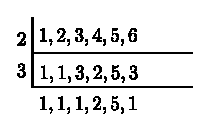
\includegraphics{images/chap8/ans30.eps}

\text{60 + 1 ಸಂಖ್ಯೆ  = 61}
\end{figure}

ಲ.ಸಾ.ಅ.  = $2\times 3\times 1\times 1\times 1\times 2\times 5 = 60$
\end{enumerate}
